\documentclass{beamer}

\usepackage{tikz}
\usepackage{multicol}

%\usetheme{}
\usetheme[progressbar=frametitle]{metropolis}
\useinnertheme{metropolis}
\useoutertheme{metropolis}
\usefonttheme{metropolis}

%for setting custom color scheme
% latexcolor.com can be used to peak colors
\definecolor{upbBlue}{RGB}{0,32,91} 
% Approximate match for Michigan State University; official colour appears too dark

\setbeamercolor{alerted text}{fg=upbBlue!50!red}
\setbeamercolor*{palette primary}{fg=upbBlue!60!black,bg=white!70!upbBlue}
\setbeamercolor*{palette secondary}{fg=upbBlue!70!black,bg=white!55!upbBlue}
\setbeamercolor*{palette tertiary}{bg=upbBlue!80!black,fg=white!45!upbBlue}
\setbeamercolor*{palette quaternary}{fg=upbBlue,bg=white!20!upbBlue}

\setbeamercolor*{sidebar}{fg=upbBlue,bg=upbBlue!75!white}

\setbeamercolor*{palette sidebar primary}{fg=upbBlue!10!black}
\setbeamercolor*{palette sidebar secondary}{fg=white}
\setbeamercolor*{palette sidebar tertiary}{fg=upbBlue!50!black}
\setbeamercolor*{palette sidebar quaternary}{fg=white!10!upbBlue}

\setbeamercolor*{titlelike}{parent=palette primary}
\setbeamercolor{frametitle}{bg=white!80!upbBlue}
\setbeamercolor{frametitle right}{bg=white!50!upbBlue}

\setbeamercolor*{separation line}{}
\setbeamercolor*{fine separation line}{}
\setbeamercolor{block body}{parent=normal text,use=block title,bg=red!0,fg=}



\title[short title]{Presentation template}
\subtitle{A template for beamer}
\author{Afshin Amini}
\institute[DICE group]{University of Paderborn, Data Science Department}


\logo{
\includegraphics[width=1.7cm]{logo.png}}

%comment next line for displaying the current date, or write in what date you want like the line after next line
\date{}
%\date{ December 2018 }



%Global Background must be put in preamble 
%\usebackgroundtemplate%
%{% \tikz\node[opacity=0.05]{\includegraphics[width=\paperwidth,height=\paperheight]{bg.png}};%
%}

\begin{document}
	
\metroset{block=fill}

{
	\usebackgroundtemplate%
	{%
		%set opacity between 0 to 100 
		\tikz\node[opacity=0.05]{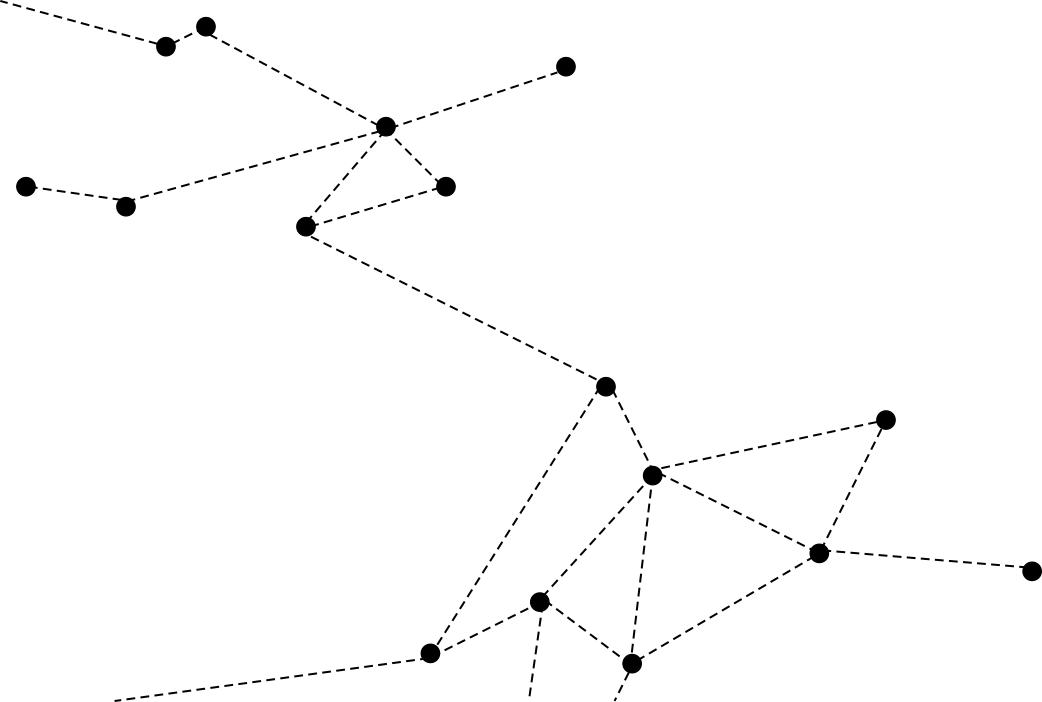
\includegraphics[width=\paperwidth,height=\paperheight]{bgTitle.png}};%
	}
\begin{frame}
\titlepage
\end{frame}
}
{
	\usebackgroundtemplate%
	{%
		%set opacity between 0 to 100
		\tikz\node[opacity=0.05]{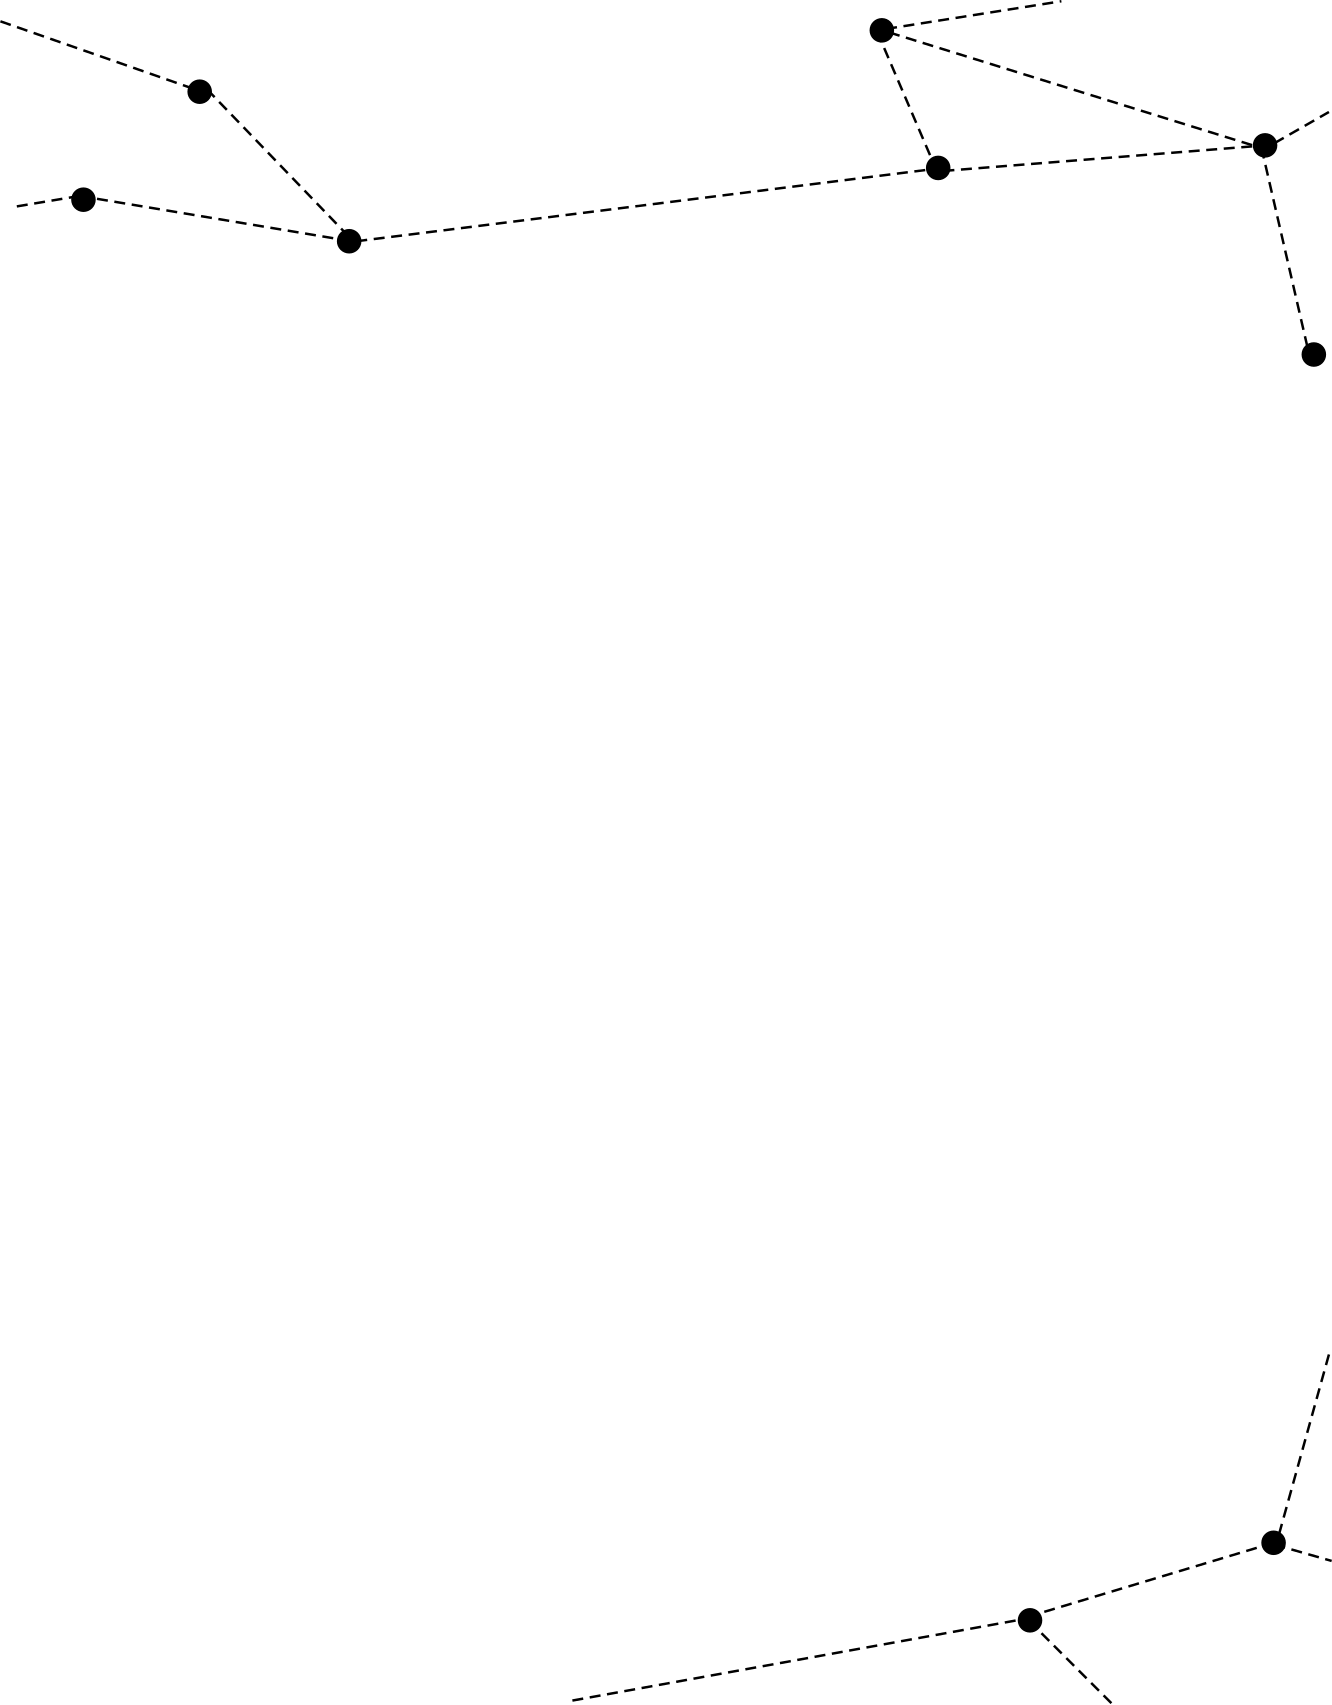
\includegraphics[width=\paperwidth,height=\paperheight]{bgAllPages.png}};%
	}
\begin{frame}
Hello World
\end{frame}	
	
\begin{frame}{Title Name of this slide}
This slide has a Title
\end{frame}	

\begin{frame}{Items List}
\begin{itemize}
	\item item1
	\item item2
\end{itemize}
\end{frame}


\begin{frame}{Enumerates List}
\begin{enumerate}
\item item1
\item item2
\end{enumerate}
\end{frame}

\begin{frame}{Custom Enumerates List}
\begin{enumerate}[(A)]
\item item1
\item item2
\end{enumerate}
\end{frame}

% By default contents are in the middle of the page to have themat the top before title of each frame we should insert [t]. In addition if you want have some margin from top you can use \vspace{} 
\begin{frame}[t]{Content at top} \vspace*{10pt}
\begin{enumerate}
	\item item1
	\item item2
\end{enumerate}
\end{frame}

\begin{frame}[t]{Alert a text} \vspace*{10pt}
This \alert{word} has been alerted.
\end{frame}

\begin{frame}[t]{Block} \vspace*{10pt}
\begin{block}{Definition of something}
The definition of \textbf{something} is given here.
\end{block}

\begin{theorem}
	\label{theorem1}
	A theorem is given here
\end{theorem}

\begin{example}
	An example of theorem \ref{theorem1} %ref is referencing to the label in definition of the previous theorem
\end{example}

\end{frame}

\begin{frame}[t]{Animation using pause command} \vspace*{10pt}

\begin{itemize}
	\item A \pause
	\item B \pause
	\item C 
\end{itemize}

\end{frame}


\begin{frame}[t]{Animation using only command in itemize} \vspace*{10pt}

\begin{itemize}
	%1-3 means from 1 to 3 is visible
	\item<1-3> A
	%2 means in only 2nd slide is visible
	\item<2> B
	%3- means from 3 to end is visible
	\item<3-> C (B is not visible from now on)
	%4 means only in 4th slide is visible
	\item<4> D (A, B are not visible in the step)
\end{itemize}

\end{frame}


\begin{frame}[t]{Animation using only command for every where} \vspace*{10pt}

What university you are working at? 
\only<1>{\line(1,0){50}}
\only<2->{\textcolor{blue}{University of Paderborn}}

\end{frame}

\begin{frame}[t]{Columns}
sin x, 2x ,3x are shown in the picture below
\vspace*{20pt}
\begin{columns}
\column{0.55\textwidth}

\begin{itemize}
	\item<2-> green line shows \textcolor{green}{sin(x)}
	\item<3-> red line shows \textcolor{red}{sin(2x)}
	\item<4-> yellow line shows \textcolor{yellow}{sin(3x)}
\end{itemize}

\column{0.45\textwidth}
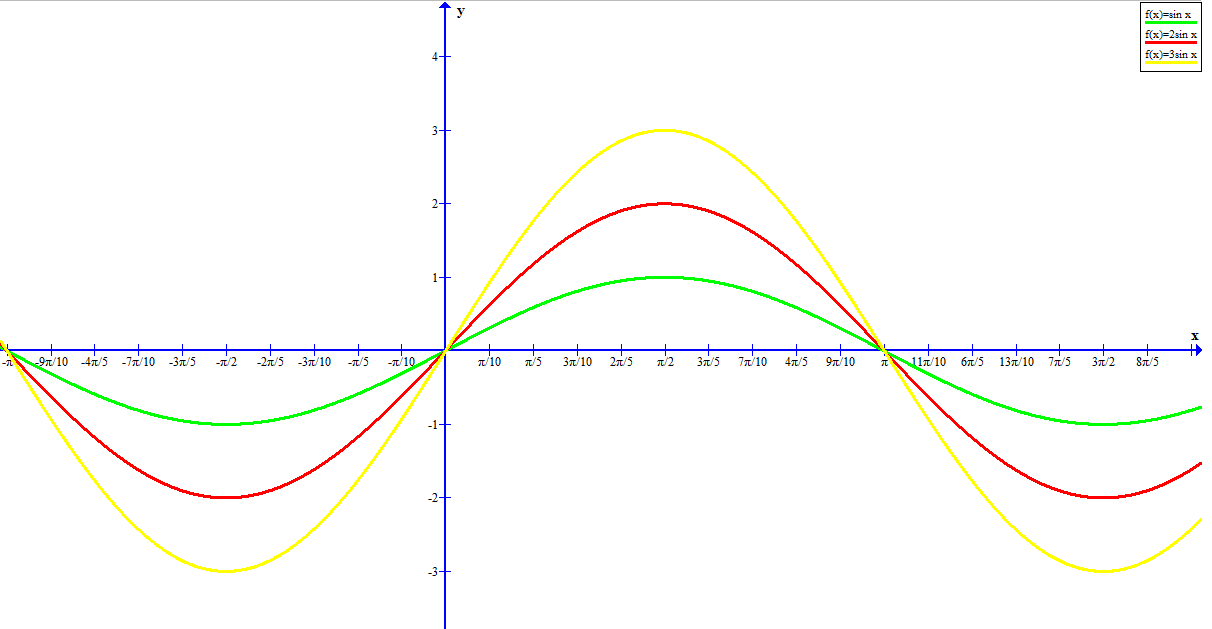
\includegraphics[scale=0.15]{sinx_2x_3x.png}
\end{columns}
\end{frame}

\begin{frame}[t]{Columns in Enumerate}\vspace{10pt}
All states of Germany
\begin{enumerate}
	\begin{multicols}{2}
	\item Baden-Württemberg
	\item Bavaria
	\item Berlin
	\item Brandenburg
	\item Bremen
	\item Hamburg 
	\item Hesse
	\item Lower Saxony
	%Note; onslide is almost like only 
	\onslide<2-> {
		\item Mecklenburg-Vorpommern
		\item \textcolor{green}{North Rhine-Westphalia}
		\item Rhineland-Palatinate
		\item Saarland
		\item Saxony
		\item Saxony-Anhalt
		\item Schleswig-Holstein
		\item Thuringia
	}
	\end{multicols}
\end{enumerate}
\end{frame}

\begin{frame}[standout]
\flushleft
The source code is available at \href{https://github.com/mnafshin/upbPresentation}{github}
\end{frame}

}
\end{document}